\documentclass[letterpaper, 11pt]{extarticle}
% \usepackage{fontspec}

% ==================================================

% document parameters
% \usepackage[spanish, mexico, es-lcroman]{babel}
\usepackage[english]{babel}
\usepackage[margin = 1in]{geometry}

% ==================================================

% Packages for math
\usepackage{mathrsfs}
\usepackage{amsfonts}
\usepackage{amsmath}
\usepackage{amsthm}
\usepackage{amssymb}
\usepackage{physics}
\usepackage{dsfont}
\usepackage{esint}

% ==================================================

% Packages for writing
\usepackage{enumerate}
\usepackage[shortlabels]{enumitem}
\usepackage{framed}
\usepackage{csquotes}

% ==================================================

% Miscellaneous packages
\usepackage{float}
\usepackage{tabularx}
\usepackage{xcolor}
\usepackage{multicol}
\usepackage{subcaption}
\usepackage{caption}
\captionsetup{format = hang, margin = 10pt, font = small, labelfont = bf}

% Citation
\usepackage[round, authoryear]{natbib}

% Hyperlinks setup
\usepackage{hyperref}
\definecolor{links}{rgb}{0.36,0.54,0.66}
\hypersetup{
   colorlinks = true,
    linkcolor = black,
     urlcolor = blue,
    citecolor = blue,
    filecolor = blue,
    pdfauthor = {Author},
     pdftitle = {Title},
   pdfsubject = {subject},
  pdfkeywords = {one, two},
  pdfproducer = {LaTeX},
   pdfcreator = {pdfLaTeX},
   }
\usepackage{titlesec}
\usepackage[many]{tcolorbox}

% Adjust spacing after the chapter title
\titlespacing*{\chapter}{0cm}{-2.0cm}{0.50cm}
\titlespacing*{\section}{0cm}{0.50cm}{0.25cm}

% Indent 
\setlength{\parindent}{0pt}
\setlength{\parskip}{1ex}

% --- Theorems, lemma, corollary, postulate, definition ---
% \numberwithin{equation}{section}

\newtcbtheorem[]{problem}{Problem}%
    {enhanced,
    colback = black!5, %white,
    colbacktitle = black!5,
    coltitle = black,
    boxrule = 0pt,
    frame hidden,
    borderline west = {0.5mm}{0.0mm}{black},
    fonttitle = \bfseries\sffamily,
    breakable,
    before skip = 3ex,
    after skip = 3ex
}{problem}

\tcbuselibrary{skins, breakable}

% --- You can define your own color box. Just copy the previous \newtcbtheorm definition and use the colors of yout liking and the title you want to use.
% --- Basic commands ---
%   Euler's constant
\newcommand{\eu}{\mathrm{e}}

%   Imaginary unit
\newcommand{\im}{\mathrm{i}}

%   Sexagesimal degree symbol
\newcommand{\grado}{\,^{\circ}}

% --- Comandos para álgebra lineal ---
% Matrix transpose
\newcommand{\transpose}[1]{{#1}^{\mathsf{T}}}

%%% Comandos para cálculo
%   Definite integral from -\infty to +\infty
\newcommand{\Int}{\int\limits_{-\infty}^{\infty}}

%   Indefinite integral
\newcommand{\rint}[2]{\int{#1}\dd{#2}}

%  Definite integral
\newcommand{\Rint}[4]{\int\limits_{#1}^{#2}{#3}\dd{#4}}

%   Dot product symbol (use the command \bigcdot)
\makeatletter
\newcommand*\bigcdot{\mathpalette\bigcdot@{.5}}
\newcommand*\bigcdot@[2]{\mathbin{\vcenter{\hbox{\scalebox{#2}{$\m@th#1\bullet$}}}}}
\makeatother

%   Hamiltonian
\newcommand{\Ham}{\hat{\mathcal{H}}}

%   Trace
\renewcommand{\Tr}{\mathrm{Tr}}

% Christoffel symbol of the second kind
\newcommand{\christoffelsecond}[4]{\dfrac{1}{2}g^{#3 #4}(\partial_{#1} g_{#2 #4} + \partial_{#2} g_{#1 #4} - \partial_{#4} g_{#1 #2})}

% Riemann curvature tensor
\newcommand{\riemanncurvature}[5]{\partial_{#3} \Gamma_{#4 #2}^{#1} - \partial_{#4} \Gamma_{#3 #2}^{#1} + \Gamma_{#3 #5}^{#1} \Gamma_{#4 #2}^{#5} - \Gamma_{#4 #5}^{#1} \Gamma_{#3 #2}^{#5}}

% Covariant Riemann curvature tensor
\newcommand{\covariantriemanncurvature}[5]{g_{#1 #5} R^{#5}{}_{#2 #3 #4}}

% Ricci tensor
\newcommand{\riccitensor}[5]{g_{#1 #5} R^{#5}{}_{#2 #3 #4}}

\begin{document}

\begin{Large}
    \textsf{\textbf{Lab 1 Prelab}}
    
    
\end{Large}

\vspace{1ex}

\textsf{\textbf{Student:}} \text{Thomas Newman}, \href{mailto:tnewman057@gmail.com}{\texttt{tnewman057@gmail.com}}\\
\textsf{\textbf{Lecturer:}} \text{Houshang Karimi}, \href{mailto:hkarimi6@yorku.ca}{\texttt{hkarimi6@yorku.ca}}


\vspace{2ex}

\begin{problem}{Voltage Division}{problem-label}
Find the voltage $V_\text{out}$ in Fig. L1.1, where $R_1$ = 4.7 K:, $R_2$ = 6.8 K$\Omega$. If a load with
resistance of 5.6K$\Omega$ is attached to the output terminal, what is the voltage of $V_\text{out}$?
\begin{figure}[H]
	\centering
	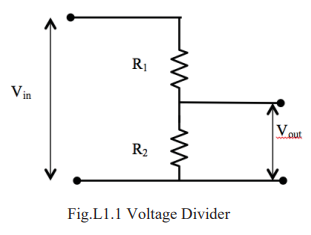
\includegraphics[width=0.46\textwidth]{fig1.png}
	\caption{Circuit for Problem 1.}
	\label{fig:cir_res3}
\end{figure}

\[R_\text{eq} = (\frac{1}{R_2} + \frac{1}{5.6k\Omega})^-1 = (\frac{1}{6.8k\Omega} + \frac{1}{5.6k\Omega})^-1 = 3.071\text{ k$\Omega$}\]
\[V_\text{out} = V_\text{in}\frac{R_\text{eq}}{R_1 + R_\text{eq}} = V_\text{in}\frac{3.071\text{ k $\Omega$}}{4.7 \text{ k $\Omega$} + 3.071 \text{ k $\Omega$}} = 0.3952 V_\text{in}\]

\end{problem}


\begin{problem}{Circuit Analysis}{problem-label-2}
Find the voltage across each resistor ($V_\text{RX}$) and the current in each resistor ($I_\text{RX}$) in Fig
L1.2. Assume the following values for the resistors: $R_1$ = 1 K$\Omega$, $R_2$ = 4.7 K$\Omega$, $R_3$ = 10
K$\Omega$, $R_4$ = 4.7 K$\Omega$, $R_5$= 1 K$\Omega$, $V_1$= 5V, $V_2$= 7V.
\begin{figure}[H]
	\centering
	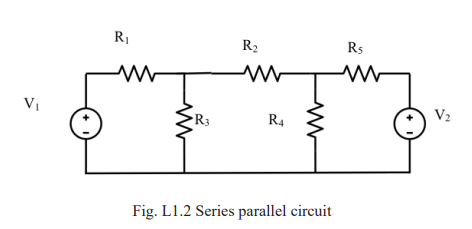
\includegraphics[width=0.46\textwidth]{fig2.png}
	\caption{Circuit for Problem 2.}
	\label{fig:cir_res3}
\end{figure}

    \[\text{KCL top left: }I_1 = I_3 + I_2\,\,\,\,\,\,\, I_3 = I_1-I_2\]
    \[\text{KCL top right: }I_4 = I_5 + I_2\]
    \[\text{KVL left mesh: } 5-1000I_1 - 10000I_3 = 0\]
    \[\text{KVL right mesh: } -7+4700I_4 +1000I_5 = 0\]
    \[\text{KVL outer loop: } -2 -1000I_1-47000I_2 + 1000I_5 = 0\]
    \[\text{Solve for $I_1$: }5-1000I_1 - 10000(I_1 - I_2) = 0\]
    \[5-1000I_1 - 10000I_1 + 10000I_2 = 0\]
    \[5 = 11000I_1 - 10000I_2\]
    \[I_1 = \frac{5+10000I_2}{11000}\]
    \[\text{Solve for $I_5$: }-7 + 4700(I_5 + I_2) + 1000I_5 = 0\]
    \[-7+5700I_5 + 4700I_2 = 0\]
    \[I_5 = \frac{7-4700I_2}{5700}\]
    \[\text{Using KVL outer loop, solve for $I_2$: } -2-1000(\frac{5+10000I_2}{11000})-4700I_2 + 1000(\frac{7-4700I_2}{5700})\]
    \[-2=(\frac{5+10000I_2}{11})+4700I_2-(\frac{7-4700I_2}{5.7})\]
    \[-2 = \frac{5}{11} + \frac{10000I_2}{11} + 4700I_2 - \frac{7}{5.7}-\frac{4700I_2}{5.7}\]
    \[-1.226 = 4700I_@ + 909.09I_2 - 824.56I_2 = 4784.53I_2\]
    \[I_2 = -0.256\text{ mA}\]
    \[I_1 = \frac{5+10000(-0.256\text{ mA}}{11000} = 22.15 \text{ mA}\]
    \[I_5 = \frac{7-4700(-0.256\text{ mA})}{5700} = 1.43 \text{ mA}\]
    \[I_4 = I_5 + I_2 = 1.43 \text{ mA} + (-0.256 \text{ mA}) = 1.18 \text{ mA}\]
    \[I_3 = I_1-I_2 = 0.2215 \text{ mA} - (-0.256 \text{ mA}) = 0.477 \text{ mA}\]
    \[V_1 = I_1R_1 = 0.2215 \text{ mA}(1000\Omega) = 0.2215 \text{ V}\]
    \[V_2 = I_2R_2 = -0.256 \text{ mA}(4700\Omega) = -1.203 \text{ V}\]
    \[V_3 = I_3R_3 = 0.477 \text{ mA}(10000\Omega) = 4.77 \text{ V}\]
    \[V_4 = I_4R_4 = 1.18 \text{ mA}(4700\Omega) = 5.55 \text{ V}\]
    \[V_5 = I_5R_5 = 1.43 \text{ mA}(1000\Omega) = 1.43 \text{ V}\]
    \[\therefore \text{$V_1$ = 0.2215 V, $V_2$ = -1.203 V, $V_3$ = 4.77 V, $V_4$ = 5.55 V, $V_5$ = 1.43 V}\]
    \[\text{$I_1$ = 0.2215 mA, $I_2$ = -0.256 mA, $I_3$ = 0.477 mA, $I_4$ = 1.18mA, $I_5$ = 1.43 mA}\]
\end{problem}



\end{document}